\documentclass[../main/main.tex]{subfiles}

\raggedbottom

\makeatletter
\renewcommand{\@chapapp}{Ondes -- chapitre}
\makeatother

% \toggletrue{student}

\begin{document}
\setcounter{chapter}{0}

\chapter{Ondes progressives}

%Tension et vitesse en fonction du milieu~: \url{https://phet.colorado.edu/sims/html/wave-on-a-string/latest/wave-on-a-string_fr.html}

\section{Introduction}
\subsection{Signal}
Les signaux constituent l'essence même de l'Univers physique.
\begin{rdefi}{\tiny Définition}
    On appelle \textbf{signal} une grandeur physique mesurable pouvant varier
    dans le temps et qui transporte une information.
\end{rdefi}
\begin{rexem}{Exemples}
    \begin{itemize}
        \item Signal \textbf{sonore}~: voix, instrument de musique~;
        \item Signal sismique~;
        \item Signal électrique…
    \end{itemize}
\end{rexem}
À noter que la notion de signal ou d'information \textbf{dépend de
l'observation}. Les ondes radio servent bien sûr à écouter la radio, mais au
départ leur découverte était perturbée par le premier signal lumineux de
l'Univers, le fonds diffus cosmologique~: il baigne la totalité de l'Univers et
est fondamental dans la cosmologie, mais peut être parasite selon l'objectif.

\subsection{Perturbation}

\begin{rdefi}{\tiny Définition}
    Une \textbf{perturbation} est une modification locale et temporaire des
    propriétés d’un milieu.
\end{rdefi}
\begin{rexem}{Exemples}
    \begin{itemize}
        \item Jet d'un caillou dans un lac~;
        \item Séisme~;
        \item Déplacement de la membrane d'un haut-parleur…
    \end{itemize} 
\end{rexem}
Une perturbation, quand elle est créée, se propage autour d'elle de proche en
proche~: chaque point impacté va subir des modifications temporaires similaires
à celle de la source. Après le passage de cette perturbation, chaque point
retrouve sa position initiale.

\subsection{Onde}
\begin{bdefi}{\tiny Définition}
    On appelle \textbf{onde} la propagation d’une perturbation, dans un milieu
    matériel ou dans le vide.
\end{bdefi}

Certaines ondes ont besoin d’un milieu matériel pour se propager~: ce sont les
ondes \textbf{mécaniques}. Les ondes sismiques, les ondes dans la corde ou les
ondes sonores en sont des exemples. Certaines ondes peuvent se propager dans le
vide, comme les ondes \textbf{électromagnétiques}. Les infrarouges, la lumière
visible ou les micro-ondes sont des exemples d’ondes électromagnétiques.

\begin{rexem}{Exemples}
    \begin{itemize}
        \item Le caillon dans le lac forme des rides qui s'éloignent du point
            d'impact, mais il n'y a \textbf{pas de mouvement d'ensemble du
            fluide}.
        \item La membrane du haut-parleur, lors de son déplacement elle provoque
            une brève \textbf{compression-dilatation} de l’air qui la touche.
            Cette propagation se déplace ensuite dans l’air~: ce sont les ondes
            sonores. Elles peuvent aussi se déplacer dans les liquides et dans
            les solides.
    \end{itemize}
\end{rexem}

\subsection{Perturbation et propagation}

La perturbation se propageant peut être soit parallèle, soit perpendiculaire à
la direction de propagation. On distingue donc~:

\begin{rdefi}{Définition}
    \begin{itemize}
        \item \textbf{Onde transversale}\footnote{\url{https://phyanim.sciences.univ-nantes.fr/Ondes/general/onde_transversale.php}}~: la perturbation est perpendiculaire à
            la direction de propagation~;
        \item \textbf{Onde longitudunale}\footnote{\url{https://phyanim.sciences.univ-nantes.fr/Ondes/general/onde_longitudinale.php}}~: la perturbation est parallèle à la
            direction de propagation.
    \end{itemize}
\end{rdefi}

\begin{rexem}{Exemples}
    \begin{minipage}{0.50\linewidth}
        \begin{itemize}
            \item \textbf{Longitudinales}~:
                \begin{itemize}
                    \item Certaines ondes sismiques~;
                    \item Contraction-élongation d'un ressort.
                \end{itemize}
        \end{itemize}
    \end{minipage}
    \hfill
    \begin{minipage}{0.48\linewidth}
        \begin{itemize}
            \item \textbf{Transversales}~:
                \begin{itemize}
                    \item Mouvement d'une corde secouée~;
                    \item Vagues sur l'eau.
                \end{itemize}
        \end{itemize}
    \end{minipage}
\end{rexem}

\section{Onde progressive à une dimension}
\subsection{Définition}
\begin{bdefi}{Définition}
    Une onde est dite \textbf{progressive} si sa propagation ne se fait que
    \textbf{dans un seul sens depuis sa source}. À un instant ultérieur, on
    retrouve la perturbation \textit{à l’identique plus loin}. \bigbreak
    Elle est dit \textbf{à une dimension} si c'est~:
    \begin{itemize}
        \item une onde qui se propage dans un milieu matériel à une dimension ;
        \item ou une onde qui se propage dans un milieu matériel à deux ou trois
            dimensions, avec une direction de propagation unique.
    \end{itemize}
\end{bdefi}

\begin{rexem}{Exemples}
    \begin{itemize}
        \item \textbf{1D}~: onde le long d'une corde, compression le long d'un
            ressort~;
        \item \textbf{2D}~: vagues sur l'eau~;
        \item \textbf{3D}~: son, lumière.
    \end{itemize}
\end{rexem}

\subsection{Représentation spatiale et célérité des ondes}
On fixe le temps et on observe le milieu dans sa dimension de propagation~:
c'est une représentation \textbf{photographique}.

\begin{rdefi}{\tiny Définition}
    Dans une représentation \textbf{spatiale}, on regarde à un \textbf{temps
    fixé} la perturbation dans \textbf{tout l’espace}. Voir cette
animation\footnote{\url{https://phyanim.sciences.univ-nantes.fr/Ondes/general/retard.php}}.
\end{rdefi}

\begin{center}
    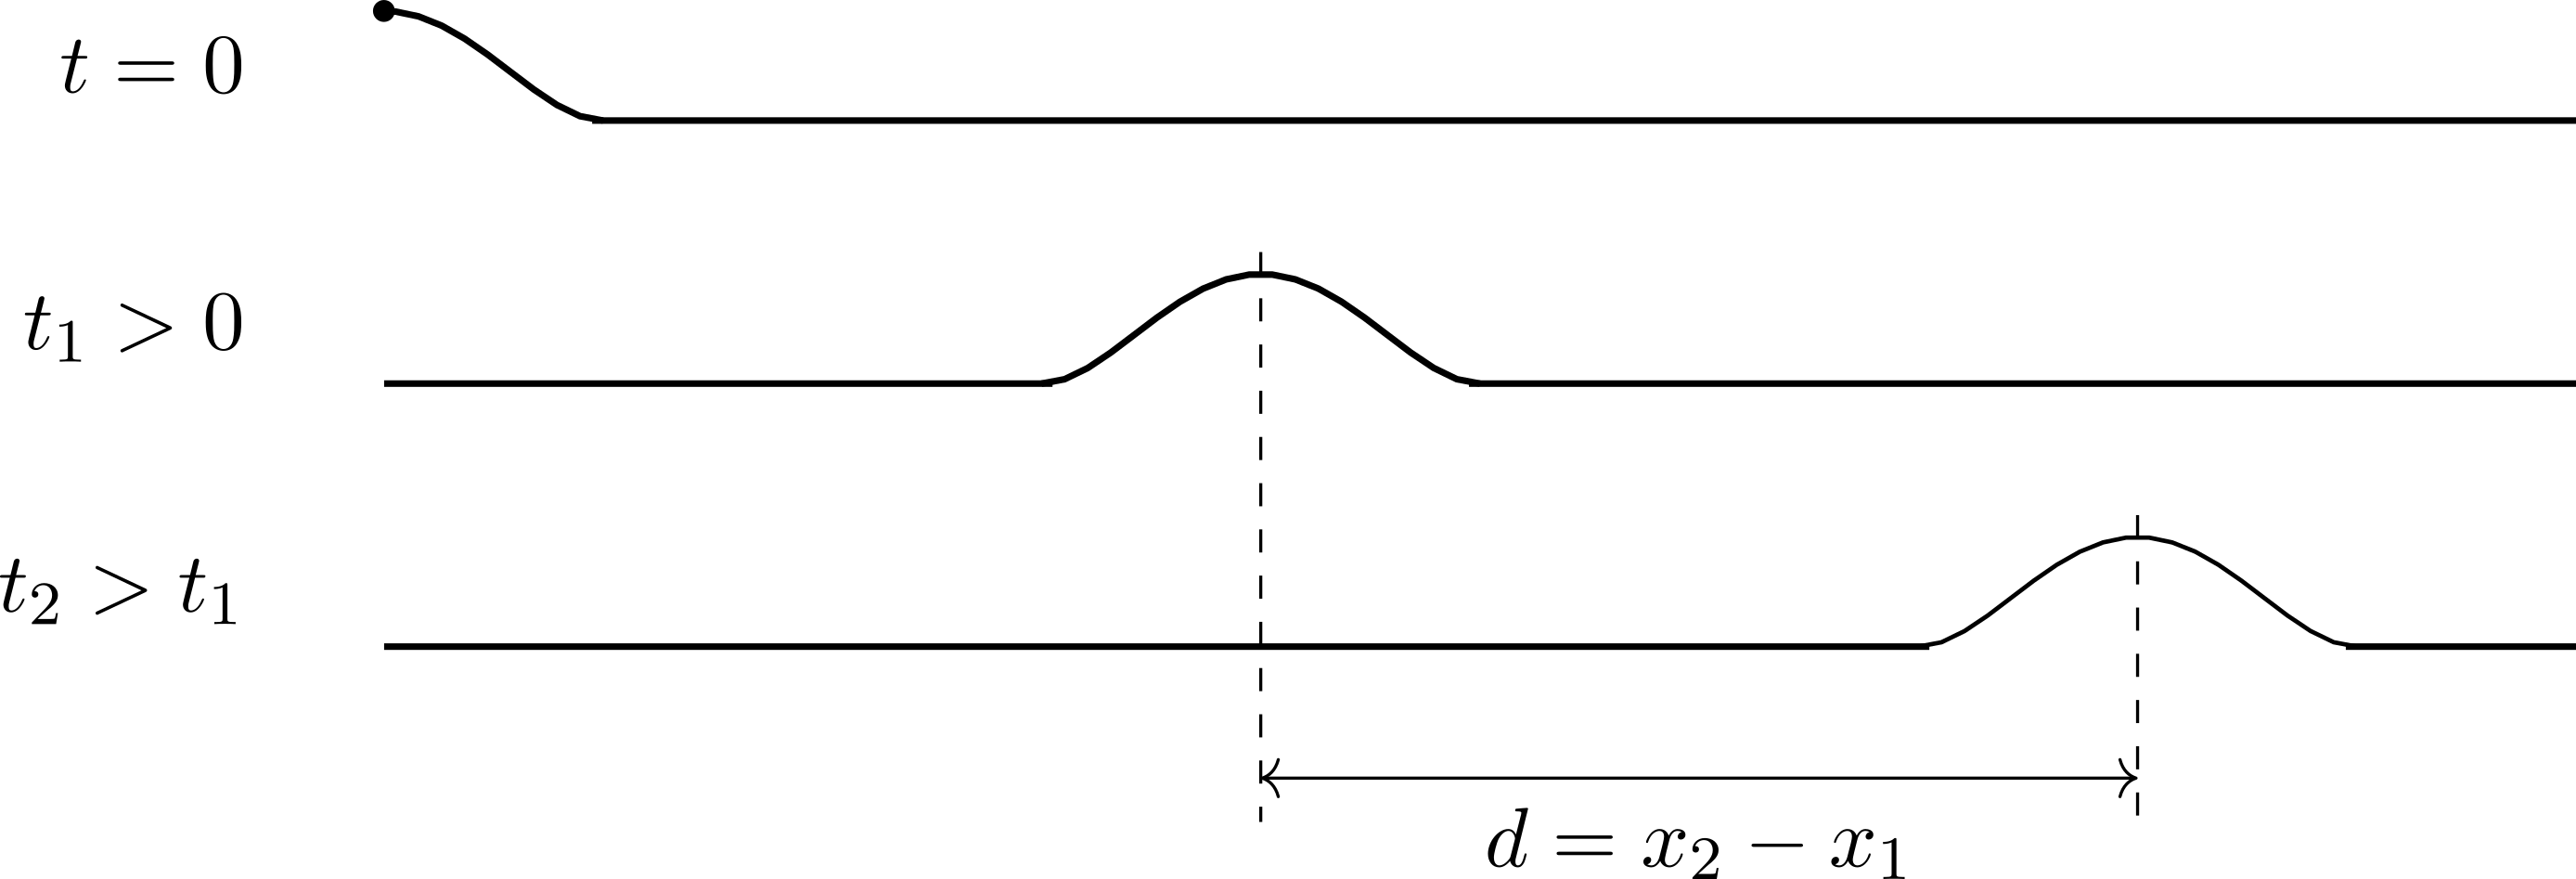
\includegraphics[width=.6\linewidth]{rep_spa}
\end{center}

Lorsqu’une onde se propage, on peut définir une vitesse de propagation de la
perturbation. Pour la distinguer de la vitesse d’un point matériel, on emploi
plutôt le terme célérité. Par convention, celle-ci est toujours positive.

\begin{bdefi}{Définition}
    La célérité $c$ d’une onde est le quotient de la distance $d$ parcourue par la
    perturbation, sur l’intervalle de temps $\Delta t$ que dure ce parcours :
    \[\boxed{c = \frac{d}{\Delta t}}\]
\end{bdefi}

Sur le schéma précédent,
\[
    c = \frac{x_2-x_1}{t_2-t_1}
\]
En première approximation, la célérité ne dépend pas de la perturbation mais
seulement de la nature et des propriétés du \textbf{milieu}.
\begin{table}[h]
    \centering
    \caption{Ordres de grandeur de célérité à connaître}
    \label{tab:ctoknow}
    \begin{tabular}{lc}
        \toprule
        Signal & Célérité
        \\\midrule
        Ondes électromagnétiques & \SI{3.0e8}{m.s^{-1}}
        \\
        Son dans l'air (\SI{20}{\degreeCelsius}, \SI{1}{bar}) & $\approx$
        \SI{340}{m.s^{-1}}
        \\
        Son dans les métaux & quelques \si{km.s^{-1}}
        \\
        Son dans l'eau & \SI{1.5}{km.s^{-1}}
        \\\bottomrule
    \end{tabular}
\end{table}

\begin{rexem}{Application}
    Un mascaret est une vague solitaire remontant un fleuve au voisinage de son
    estuaire, et provoqué par une interaction entre son écoulement et la marée
    montante. On considère ici un mascaret qui se déplace à la vitesse $c =
    \SI{18}{km.h^{-1}}$ le long d'un fleuve rectiligne, et on définit un axe
    $(Ox)$ dans la direction du sens de sa propagation.

    À l'instant $t=0$, le profil du niveau de l'eau du fleuve a l'allure
    suivante~:
    \begin{center}
        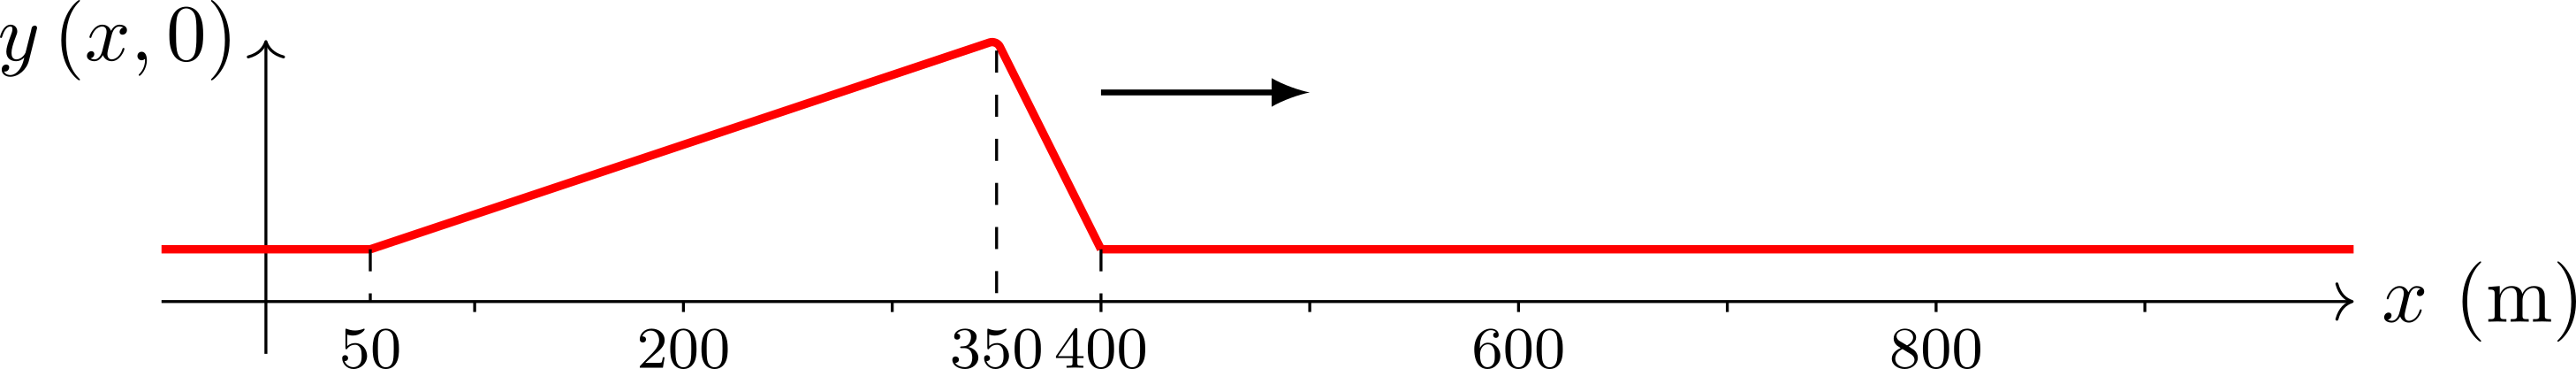
\includegraphics[width=0.8\linewidth]{rep_spa-masc_a}
    \end{center}
    Faire un schéma du profil du fleuve à $\tau = \SI{1}{min}$ en supposant que
    l'onde se propage sans déformation.
    \cswitch{white}{
        La queue de la vague est à $x_{q,0} = \SI{50}{m}$. À $\tau =
        \SI{1}{min}$, elle est en $x_{q,1}$. Par définition de la célérité,
        \begin{gather*}
            \frac{x_{q,1}-x_{q,0}}{\tau-0} = c
            \Leftrightarrow
            x_{q,1} = x_{q,0} + c\tau = \SI{350}{m}
    \end{gather*}}
    \cswitch{white}{
        On procèderait de même pour repérer le haut de la vague et sa tête~: en
        réalité, chaque point du mascaret se déplace de $c\tau = \SI{300}{m}$
    vers la droite.}
    \switch{
    \begin{center}
        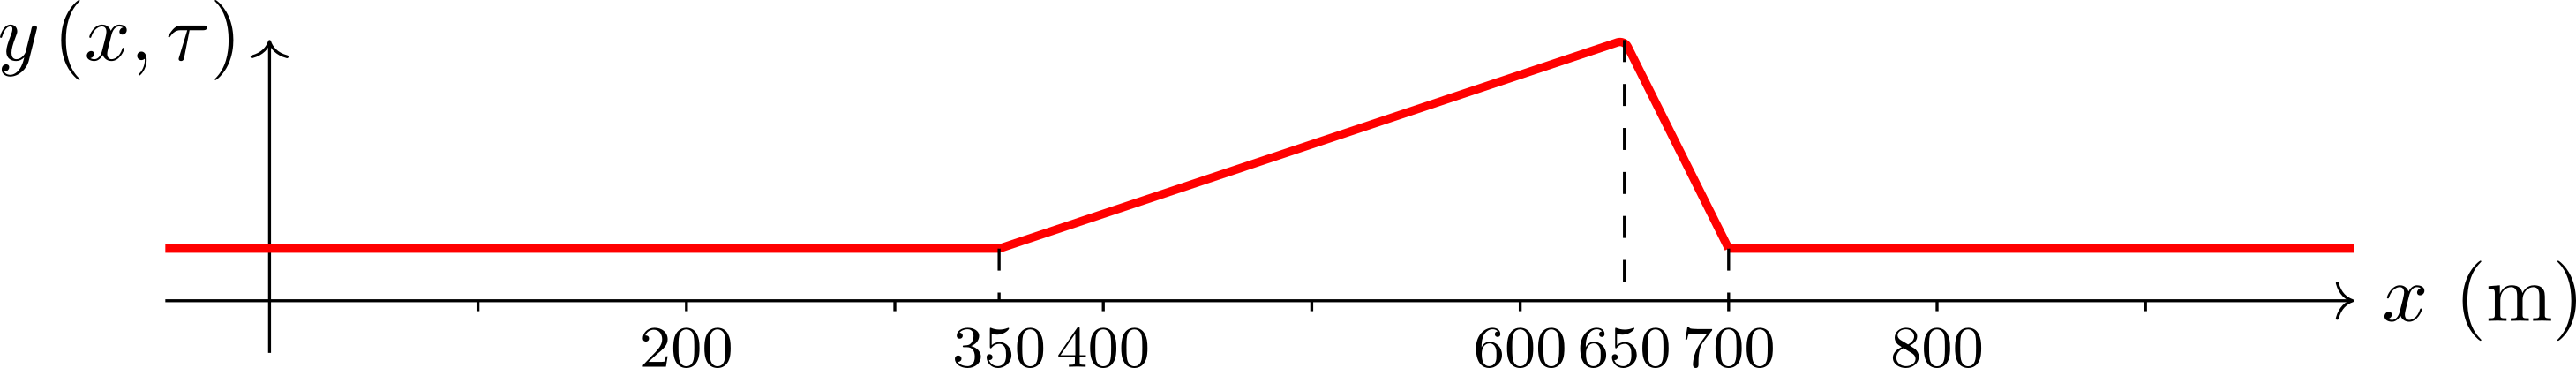
\includegraphics[width=0.8\linewidth]{rep_spa-masc_b}
    \end{center}}
    {\vspace{2cm}}
\end{rexem}

\subsection{Représentation temporelle et retard}

\begin{rdefi}{\tiny Définition}
    \cswitch{white}{Dans une représentation \textbf{temporelle}, on regarde à un
    \textbf{endroit fixé} la perturbation \textbf{sur sa durée}. Voir cette
    animation\footnote{\url{https://phyanim.sciences.univ-nantes.fr/Ondes/general/evolution_temporelle.php}}.}
\end{rdefi}

On crée à l’instant $t = 0$ une déformation à un endroit $M$. Cette perturbation se
propage le long de la corde avec une célérité $c$. Elle parvient en un point
$M_0$, situé à une distance $D$ de $M$ à~:
\cswitch{white}{\[t_1 = \frac{\rm MM'}{c}\]}

\begin{bdefi}{Définition}
    \cswitch{white}{
        La grandeur $\tau$ est le retard du point M' par rapport au point M~:
        \[\tau = \frac{\rm MM'}{v}\]
        avec $v$ la célérité de l'onde.}
\end{bdefi}

\begin{rexem}{Application}
    On reprend l’exemple de la vague précédente.
    \begin{enumerate}
        \item À quel instant la vague arrive-t-elle au point d'abscisse $x_1 =
            \SI{2.2}{km}$~? \smallbreak
            \cswitch{white}{
                À $t=0$, la tête de la vague est à $x_0 = \SI{400}{m}$. Elle
                arrive en $x_1$ avec un retard~:
                \[t = \frac{x_1-x_0}{c} = \SI{6}{min}\]
            }
        \item Un détecteur fixe, enregistrant la hauteur du fleuve en fonction
            du temps, est placé à l'abscisse $x_d = \SI{1.6}{km}$. Dessiner
            l'allure des variations $y(x_d,t)$ en fonction du temps à cette
            abscisse.
            \cswitch{white}{
            La tête de la vague arrive avec un retard~:
            \[\tau_{\text{tête}} = \frac{x_d - x_{t,0}}{c} = \SI{4}{min}\]
            Le haut de la vague arrive avec un retard~:
            \[\tau_{\text{haut}} = \frac{x_h - x_{h,0}}{c} =
            \SI{4}{min}\SI{10}{s}\]
            La queue de la vague arrive avec un retard~:
            \[\tau_{\text{queue}} = \frac{x_q - x_{q,0}}{c} =
            \SI{5}{min}\SI{10}{s}\]
            }
    \end{enumerate}
    \switch{
    \begin{center}
        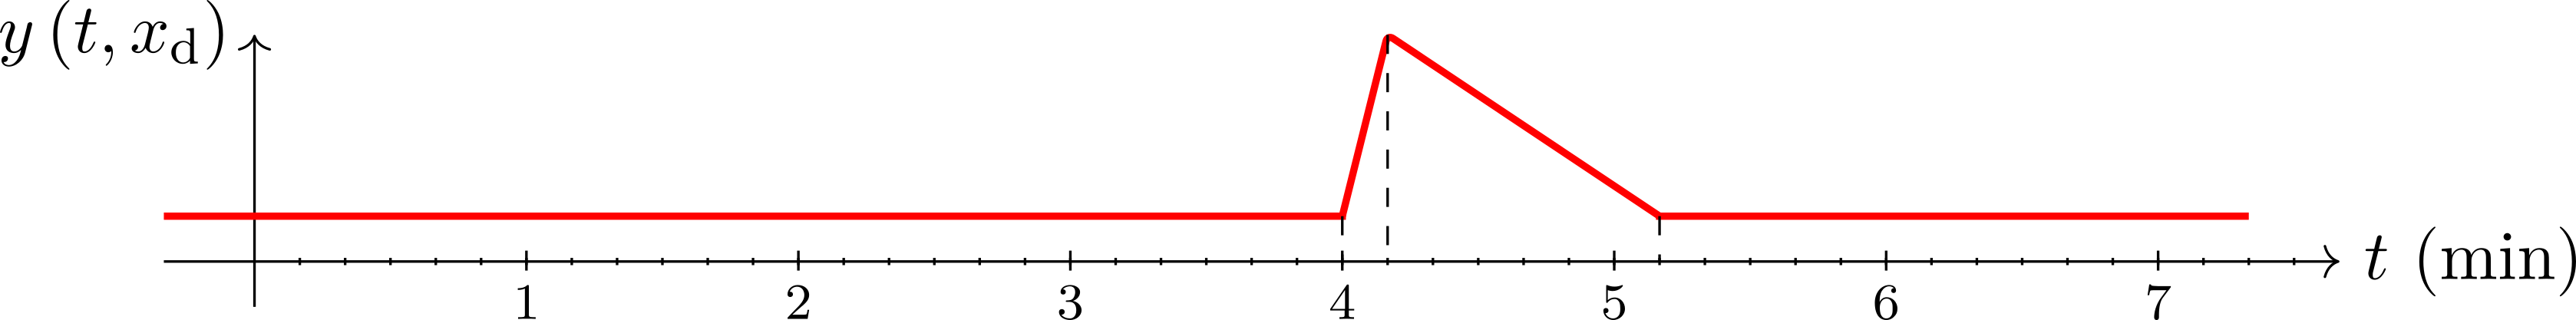
\includegraphics[width=0.8\linewidth]{rep_temp_masc}
    \end{center}}
    {\vspace{2cm}}
\end{rexem}

\subsection{Lien entre les représentations}
Nous avons vu deux représentations graphiques différentes, une selon l'espace et
une selon le temps. En réalité, le signal d'une onde est une fonction de
\textbf{deux} variables~:
\[y(x,t)\]
Pour obtenir l'une au l'autre des représentations, on fixe l'une des variables.
Une animation sur les représentations temporelles et spatiales est disponible au
lien suivant~: \url{https://www.geogebra.org/m/RkmRF9M6}

\subsection{Formes mathématiques des représentations}
\subsubsection{À partir de la représentation spatiale}
L'onde observée à $t=0$ se déplace vers la droite. À l'instant $t$, elle est
décalée vers la droite de $\delta = ct$~: la valeur de $y(x,t)$ en $x$ et à
l'instant $t$ était en $x-ct$ à l'instant $t=0$, soit~:
\cswitch{white}{
    \[
        y(x,t) = y(x-ct,0)
    \]
}
On note alors $f(x) = y(x,0)$~: c'est la représentation spatiale de l'onde à
$t=0$. On a alors
\cswitch{white}{
    \[\boxed{
        y(x,t) = f(x-ct)
    }\]
}\vspace{-20pt}
\subsubsection{À partir de la représentation temporelle}

Lorsqu’une onde se propage sans atténuation ni déformation, les valeurs
observées en $x = 0$ au cours du temps sont aussi observées en $x > 0$ mais avec
un retard \cswitch{white}{$\tau = \DS\frac{x}{c}$}\!\!\!\! lié à la propagation.
La valeur de $y(x, t)$ en $x$ à l’instant $t$ était en $x = 0$ plus tôt, à
l’instant $t - x/c$. Ainsi,
\cswitch{white}{
    \[
        y(x,t) = y(0,t-\frac{x}{c})
    \]
}
La fonction $y(0,t)$ est la hauteur de la perturbation en $x=0$ à l'instant
$t$~: c'est la perturbation imposée par la source. On la note alors $g(t) =
y(0,t)$~: c'est la représentation temporelle de l'onde à $x=0$. On a alors
\cswitch{white}{
    \[\boxed{
        y(x,t) = g(t-\frac{x}{c})
    }\]
}

\begin{brorside}{Conclusion}
    La représentation temporelle en $x_0$ est le graphique de la fonction $t
    \mapsto y(x_0,t)$, soit~:
    \[t\mapsto f(x_0-ct) = g\left(t - \frac{x_0}{c}\right)\]
    \tcblower
    La représentation spatiale en $t_0$ est le graphique de la fonction $x
    \mapsto y(x,t_0)$, soit~:
    \[x\mapsto f(x-ct_0) = g\left(t_0 - \frac{x}{c}\right)\]
\end{brorside}

Si l'onde se propage vers la gauche, le raisonnement est le même~: on remplace
$x-ct$ par $x+ct$, et $t-x/c$ par $t+x/c$.

\section{Onde progressive sinuso\"idale}
\subsection{Définition}

\begin{rdefi}{\tiny Définition}
    \cswitch{white}{
        Une onde progressive est dite sinusoïdale si la source impose une
        \textbf{perturbation sinusoïdale} au milieu.
    }
\end{rdefi}

Si on relie un haut-parleur à un GBF délivrant une tension sinusoïdale, on
observe le mouvement périodique dont est animé la membrane de l’air, qui génère
une perturbation périodique de l’air.

L’exemple du diapason étudié au DS03 est également une onde progressive
sinusoïdale : lorsque l’on frappe le diapason, celui-ci vibre a une fréquence
bien déterminée, qui se propage ensuite dans l’air pour parvenir à nos oreilles.

\subsection{Double périodicité spatiale et temporelle}
\subsubsection{Observations sur l'animation \texttt{Geogebra}}
\vspace{-20pt}
\cswitch{white}{
    \begin{itemize}
        \item Lorsque l’on impose une excitation sinusoïdale, la représentation
            spatiale est aussi sinusoïdale.
        \item À célérité constante, lorsque la fréquence de l’excitation
            augmente (la période diminue), la période spatiale diminue.
        \item À fréquence de l’excitation constante, si on augmente la célérité,
            la période spatiale diminue.
    \end{itemize}
}
\vspace{-10pt}

\subsubsection{Périodicité temporelle}
Si la perturbation créée en S est sinusoïdale avec une période $T$, alors l’onde
en M l’est également (il n’y a qu’un retard entre les deux dû à la propagation).

\subsubsection{Périodicité spatiale}

Au moment de l’émission du deuxième maximum, le premier maximum a déjà parcouru
une distance $cT$. L’écart entre deux maximum successifs est la période spatiale
soit :
\[\lambda = cT\]

\begin{bprop}{Bilan}
    \cswitch{white}{
        Une onde progressive sinusoïdale présente à la fois une périodicité
        spatiale et une périodicité temporelle. La période temporelle $T$ et la
        période spatiale, nommée longueur d’onde et notée $\lambda$, sont
        reliées par la relation
        \[\boxed{\lambda = cT = \frac{c}{f}}\]
        avec $c$ la célérité de l'onde.
}
\end{bprop}

Cette relation ne vous est sûrement pas inconnue~: c'est de cette manière qu'on
définit à la fois la fréquence (temporelle) et la période (spatiale) d'une onde
électromagnétique, donnant les domaines connus rappelés ci-dessous~:

\begin{center}
    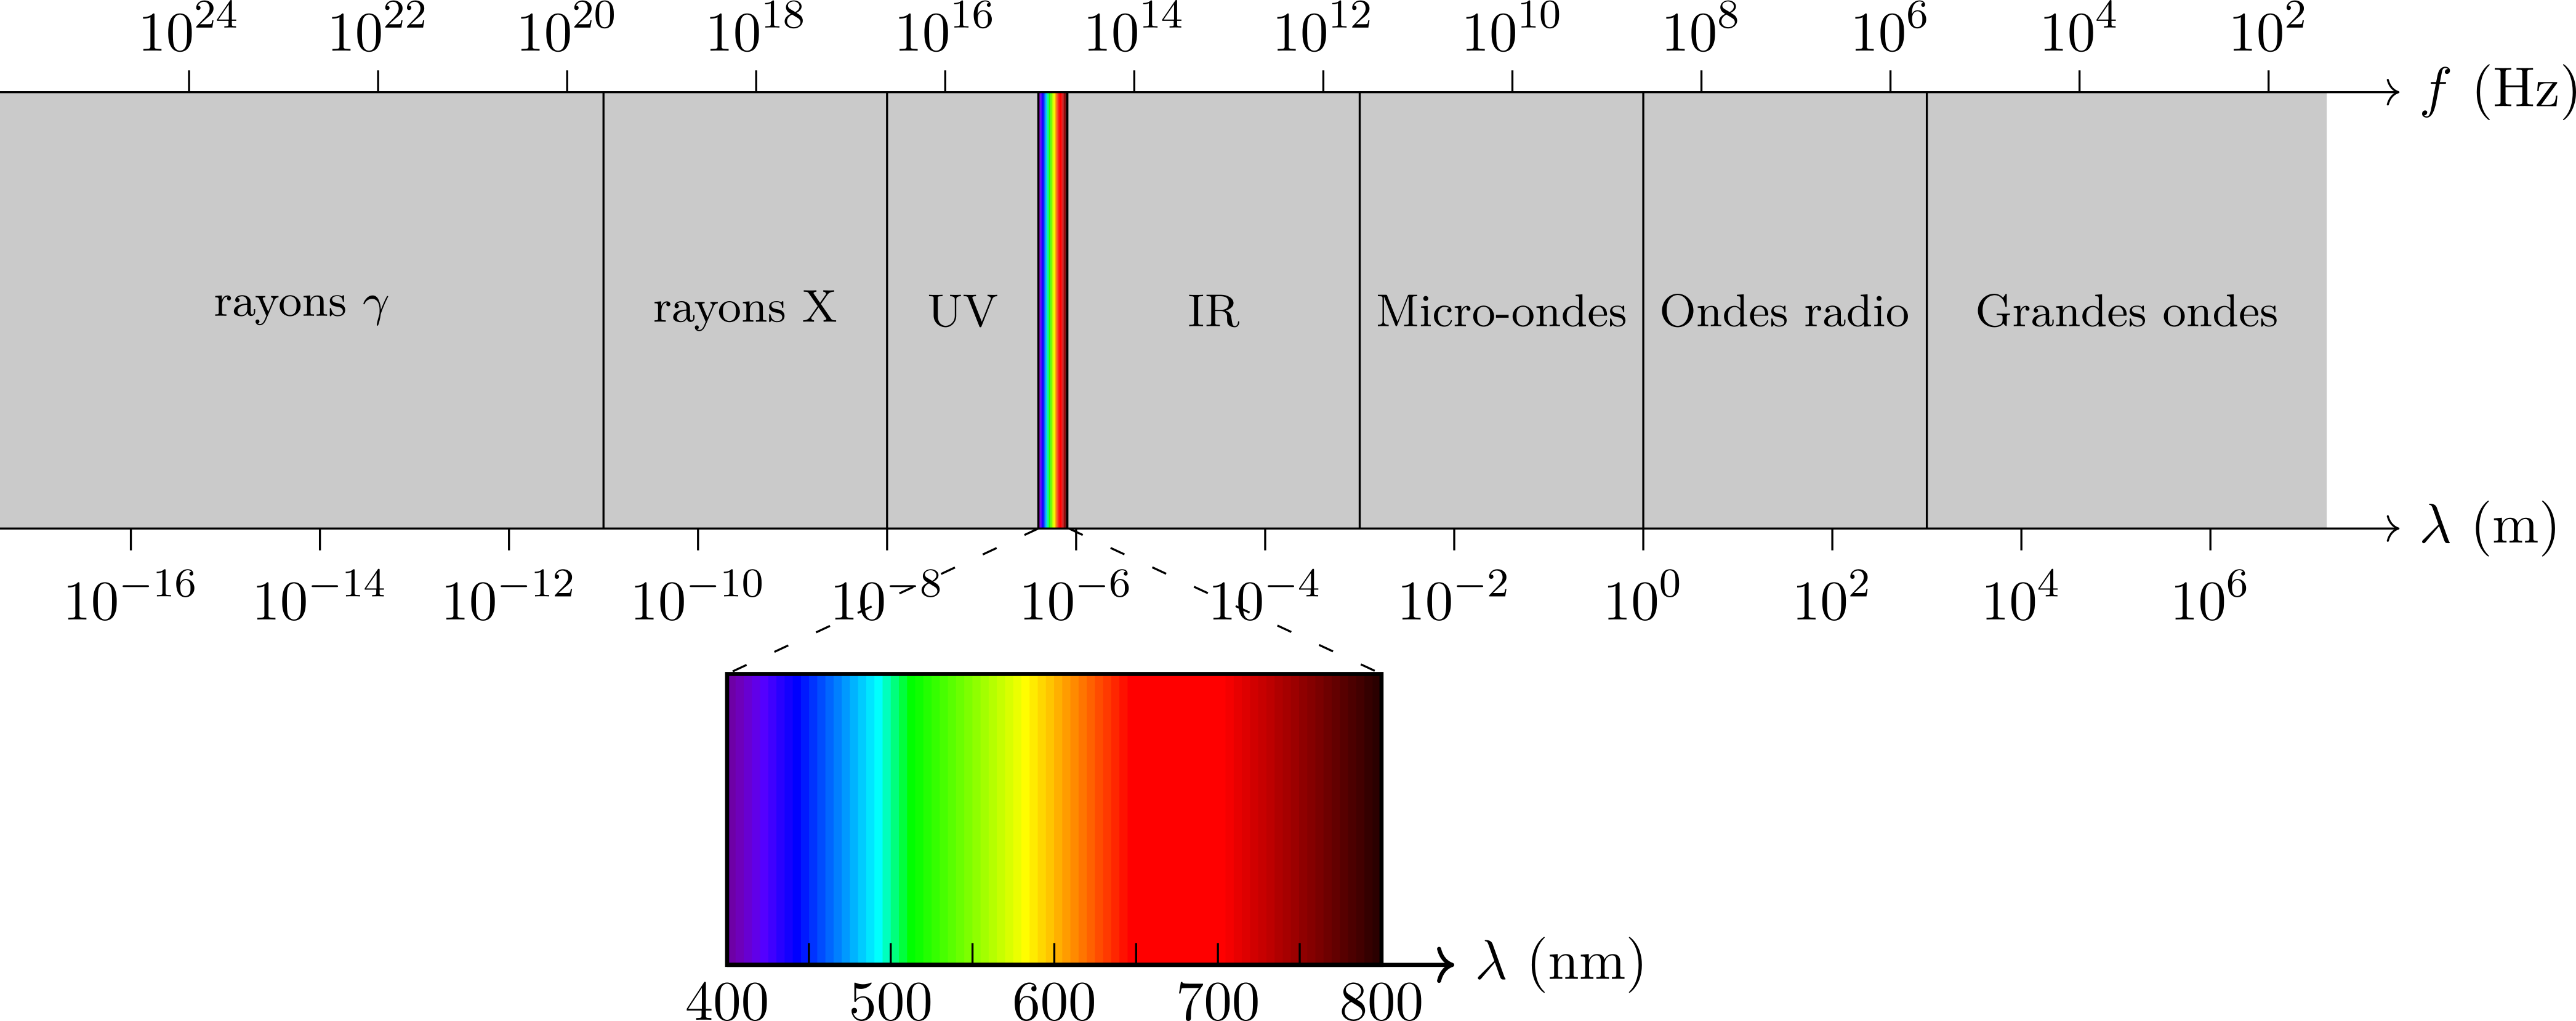
\includegraphics[width=.8\linewidth]{oem}
\end{center}

\subsection{Expression mathématique de l'onde progressive sinusoïdale}

Par définition, la perturbation $g(t)$ imposée en $x=0$ est un signal
sinusoïdal~:
\[\cswitch{white}{g(t) = A\cos(\wt+\f)}\]
Ainsi,
\cswitch{white}{
    \begin{gather*}
        s(x,t) = A\cos\left(\w\left(t - \frac{x}{c}\right) +\f\right)\\
        s(x,t) = A\cos\left(\wt - \frac{\w}{c}x +\f\right)\\
        s(x,t) = A\cos\left(\wt - \frac{2\pi}{cT}x +\f\right)
    \end{gather*}
}
\begin{bdefi}{Définition}
    Comme pour la fréquence et la pulsation, on relie la longueur d'onde à une
    autre grandeur permettant une expression simple dans une fonction
    sinusoïdale~: le \textbf{vecteur d'onde} $k$, tel que
    \[\cswitch{white}{\boxed{k = \frac{2\pi}{\lambda} = \frac{\w}{c}}
    \qavec
    k\quad\text{en}\quad\boxed{\si{rad.m^{-1}}}}\]
\end{bdefi}
\begin{bprop}{Propriété}
    L'expression générale d'une onde progressive sinusoïdale se propageant sans
    déformation ni atténuation est~:
    \cswitch{white}{
        \begin{gather*}
            \boxed{s(x,t) = A\cos \left(\wt - kx + \f \right)}\\
            \Leftrightarrow
            s(x,t) = A\cos \left( \frac{2\pi}{T}t - \frac{2\pi}{\lambda}x + \f
            \right)
        \end{gather*}
    }
    \vspace{-10pt}
\end{bprop}

\begin{rexem}{Application}
    On peut vérifier la double périodicité de l'onde ($T$ et $\lambda$). Vérifer
    par exemple la périodicité spatiale.
    \cswitch{white}{
        \begin{align*}
            s(x+\lambda,t) &= A\cos(\wt - k(x+\lambda) + \f)\\
            \Leftrightarrow
            s(x+\lambda,t) &= A\cos\left(\wt - kx - \frac{2\pi}{\lambda}\lambda +
            \f\right)\\
            \Leftrightarrow
            s(x+\lambda,t) &= A\cos(\wt - kx -2\pi +\f)\\
            \Leftrightarrow
            s(x+\lambda,t) &= A\cos(\wt - kx +\f)\\
            \Leftrightarrow
            s(x+\lambda,t) &= A\cos(\wt - kx +\f)\\
            \Leftrightarrow
            \Aboxed{
            s(x+\lambda,t) &= s(x,t)
            }
        \end{align*}
    }\vspace{-20pt}
\end{rexem}

\subsection{Vitesse de phase}

Soit une onde progressive sinusoïdale. La \textbf{phase} de l'onde est, par
définition, le terme à l'intérieur de la fonction~: $\wt-kx+\f$. Cette phase
varie spatialement et temporellement, de manière corrélée. Si on trouve une
phase mesurée en $x_1$ à l'instant $t_1$, le signal aura la même phase en $x_2$
à un instant $t_2$ donnés par la \textbf{vitesse de phase}, notée $v_\f$, telle
que~:
\vspace{-10pt}
\cswitch{white}{\[\boxed{v_\f = \frac{x_2-x_1}{t_2-t_1}}\]}
\vspace{-10pt}
\begin{bdemoside}{{\small Démonstration}\includehand{-90}{0.8cm}}
    \vspace{-10pt}
    \cswitch{white}{
        \begin{gather*}
            \wt_2-kx_2+\f = \wt_1-kx_1+\f\\
            \Leftrightarrow
            \w(t_2-t_1) = k(x_2-x_1)\\
            \Leftrightarrow
            \boxed{v_\f = \frac{x_2-x_1}{t_2-t_1} = \frac{\w}{k}}
        \end{gather*}
    }
    \tcblower
    \centering
    \cswitch{white}{
        Naturellement, la vitesse de phase s'exprime en \fbox{\si{m.s^{-1}}}.
    }
    \vspace{-10pt}
\end{bdemoside}

\section{Milieux dispersifs}

\begin{rdefi}{Définition}
    Un milieu est dit \textbf{dispersif} si\cswitch{white}{la célérité $c$
    dépend de la fréquence ou de la longueur d'onde.}
    \bigbreak
    Si c'est le cas, les différentes composantes spectrales d'un signal ne vont
    pas à la même vitesse, et donc le signal peut se déformer lors de la
    propagation.
\end{rdefi}
\begin{rexemside}{Exemples}
    {\centering\bfseries Propagation non-dispersive}
    \cswitch{white}{
    \begin{itemize}
        \item Propagation des ondes acoustiques dans un fluide. La célérité
            est~:
            \[c = \frac{1}{\sqrt{\rho_0\chi_0}}\]
            avec $\rho_0$ la masse volumique du fluide au repos et $\chi_0$ sa
            compressibilité.
        \item Propagation des ondes électromagnétiques dans le vide~:
            \[c = \SI{299792458}{m.s^{-1}}\]
            C'est une des constantes fondamentales de la physique.
    \end{itemize}
    }
    \tcblower
    {\centering\bfseries Propagation dispersive}
    \cswitch{white}{
    \begin{itemize}
        \item Propagation des ondes à la surface de l'eau. On a
            \[\w^2 = gk
                \qsoit
                v_\f = \sqrt{\frac{g}{k}}
            \]
            Ainsi, la vitesse de phase dépend de $k$, et donc de la longueur
            d'onde.
        \item Propagation des ondes électromagnétiques dans le verre~:
            \[v_\f = \frac{c}{n(\lambda)}\]
            avec $n(\lambda) = A + \frac{B}{\lambda^2}$. C'est la dispersion qui
            cause la décomposition spectrale de la lumière par un prisme.
    \end{itemize}
    }\vspace{-10pt}
\end{rexemside}

\sidecaptionvpos{figure}{c}
\begin{SCfigure}[1][h!]
    \centering
    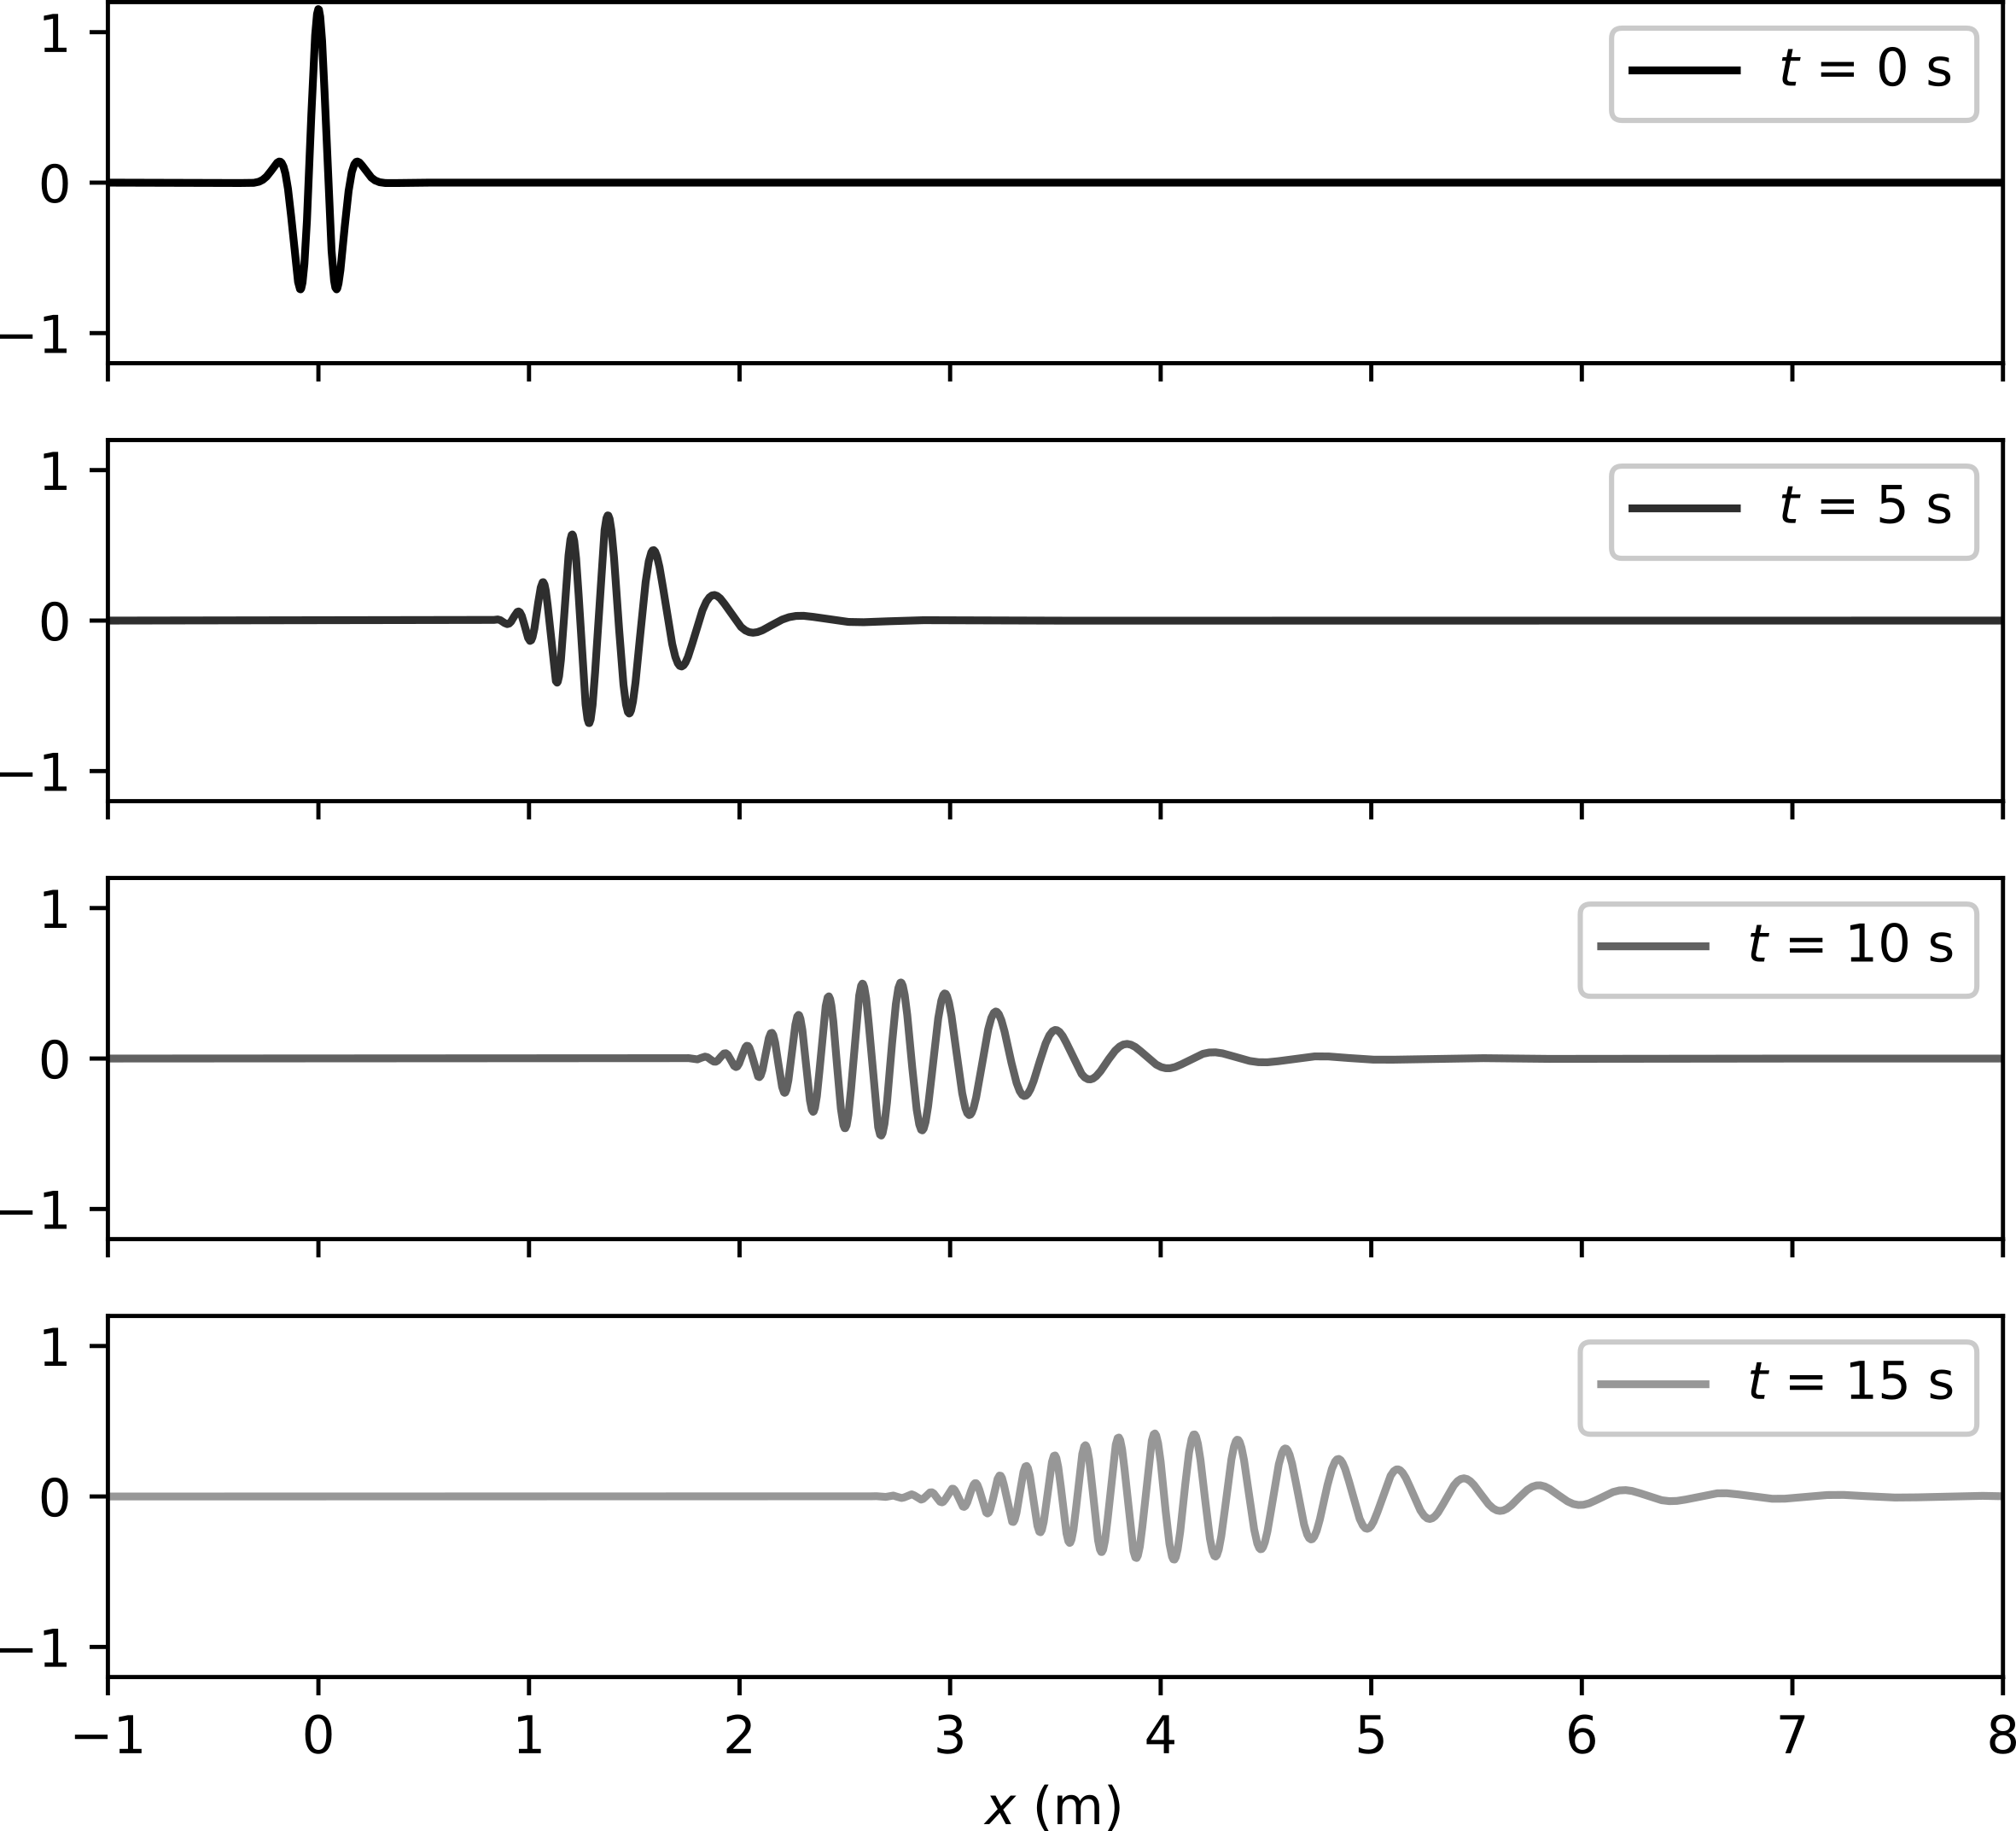
\includegraphics[width=.45\linewidth]{dispersion}
    %\captionsetup{justification=centering}
    \caption[Dispersion d'une onde à la surface de l'eau]{Propagation dispersive
        d’une onde à la surface de l’eau. On observe nettement que les
        composantes sinusoïdales de hautes fréquences se propagent avec une
        moins grande vitesse que les composantes de basses fréquences. En
    ordonnée, l’unité de la hauteur d’eau est arbitraire.}
    \label{fig:disp_eau}
\end{SCfigure}

\end{document}
